\chapter{Ряд Фурье}
\label{ch:intro}

Ряд Фурье — это способ представить периодическую функцию в виде суммы простых гармонических колебаний 
(синусов и косинусов) с разными частотами, амплитудами и фазами. \\

Функции $\{1, cos(x), sin(x), cos(2x), sin(2x) и т.д\}$ являются базисом пространтсва периодических функций (как в линейной алгебре
есть базис, допустим, трехмерного пространтсва, который состоит из ортов i, j и k, и все вектора в этом пространстве могут быть
разложены по этим ортам, т.е представлены в виде их линеной комбинации), поэтому почти любую периодическую функцию можно представить
в виде суммы функций, принадлежащих этому базису. \\

Еще одним примером разложения является ряд Тейлора. Базисом для пространства функций является множество функций $\{1, x, x^2, x^3, \dots\}$,
по которому также можно разложить почти любую функцию, т.е. представить в виде линейной комбинации многочленов.

Ряд Фурье и его коэффициенты вычисляются следующим образом:

\begin{figure}[ht]
    \centering
    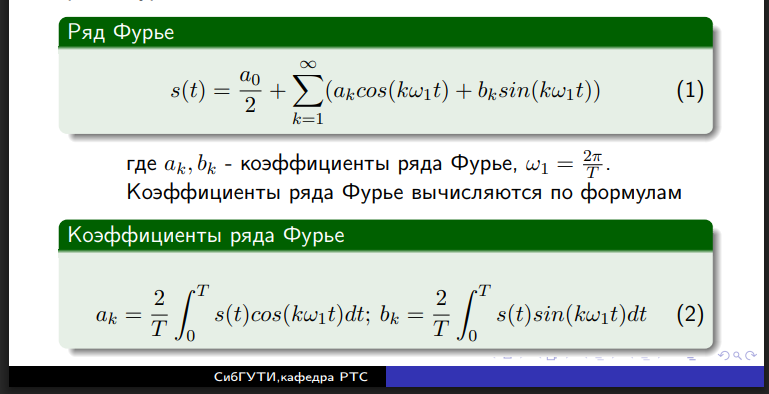
\includegraphics[width=1.0\textwidth]{furie_formula.png}
    \caption{Формула ряда Фурье и коэффициентов}
\end{figure}

где $\frac{a_0}{2}$ "--- постоянная составляющая (или среднее значение сигнала), \\
$a_k$ и $b_k$ "--- коэффициенты ряда Фурье, $a_k$ отвечает за амплитуды чётных (симметричных) составляющих функции
и показывают, насколько сильно в сигнале выражена компонента вида cos($\omega_0t$), а $b_k$ отвечает за амплитуды нечётных (асимметричных) составляющих функции
и показывают, насколько сильно в сигнале выражена компонента вида sin($\omega_0t$). \\
$k$ "--- номер гармоники ($k = 1,2,3,4,\dots$), \\
$\cos(k\omega_1 t)$ и $\sin(k\omega_1 t)$ "--- базисные функции.

Важно заметить, что сигнал, который нужно разложить в ряд Фурье, должен содержать только гармонники с частотой кратной $w_1$. Если
такое условие не выполняется, то сигнал не будет периодическим и разложить его в классический ряд Фурье невозможно.

Пример вычисления коэффициентов ряда Фурье:

\begin{figure}[H]
    \centering
    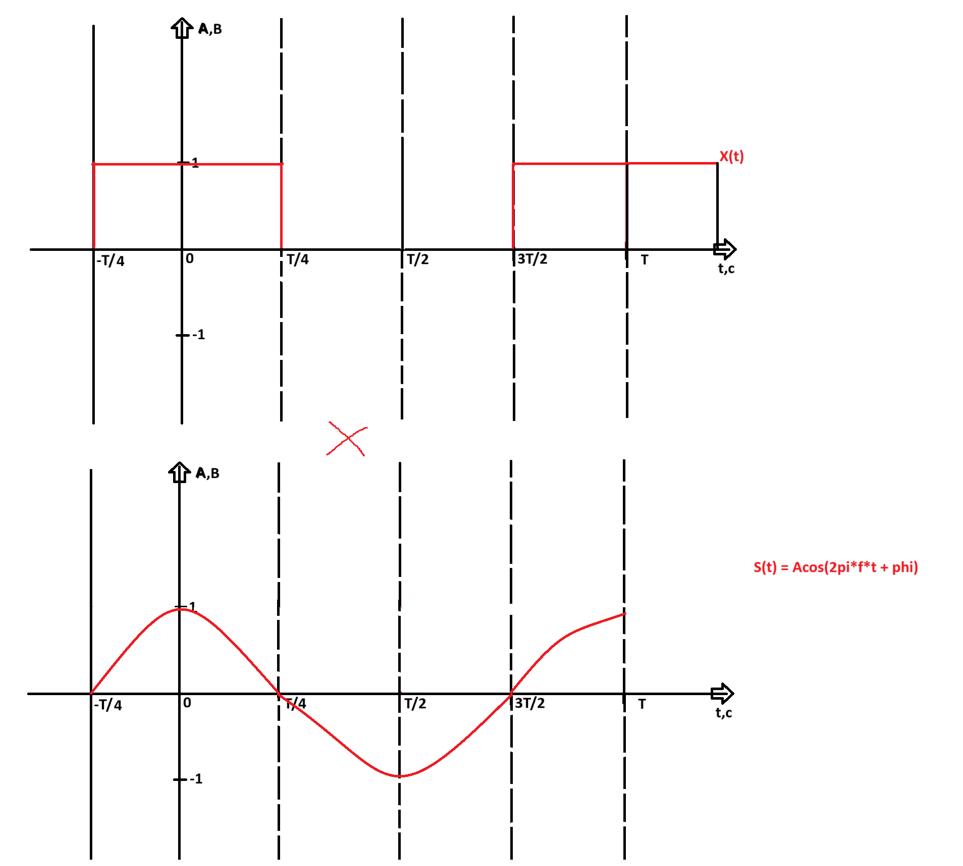
\includegraphics[width=1.0\textwidth]{a_comp_1.png}
    \caption{Геометрическая интерпретация вычисления $a_k$}
\end{figure}


\begin{figure}[H]
    \centering
    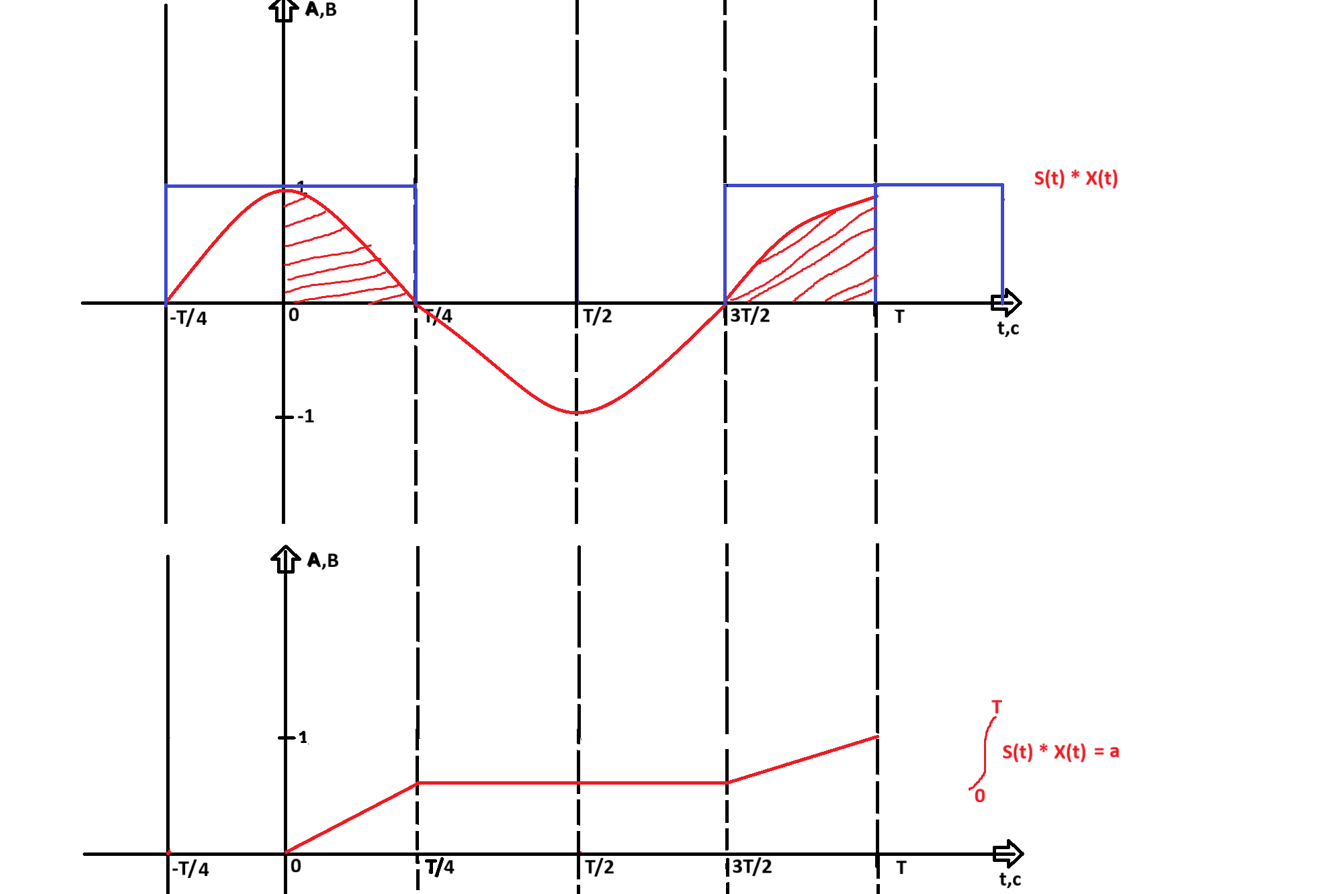
\includegraphics[width=1.0\textwidth]{a_comp_2.png}
    \caption{Геометрическая интерпретация вычисления $a_k$}
\end{figure}

\begin{figure}[H]
    \centering
    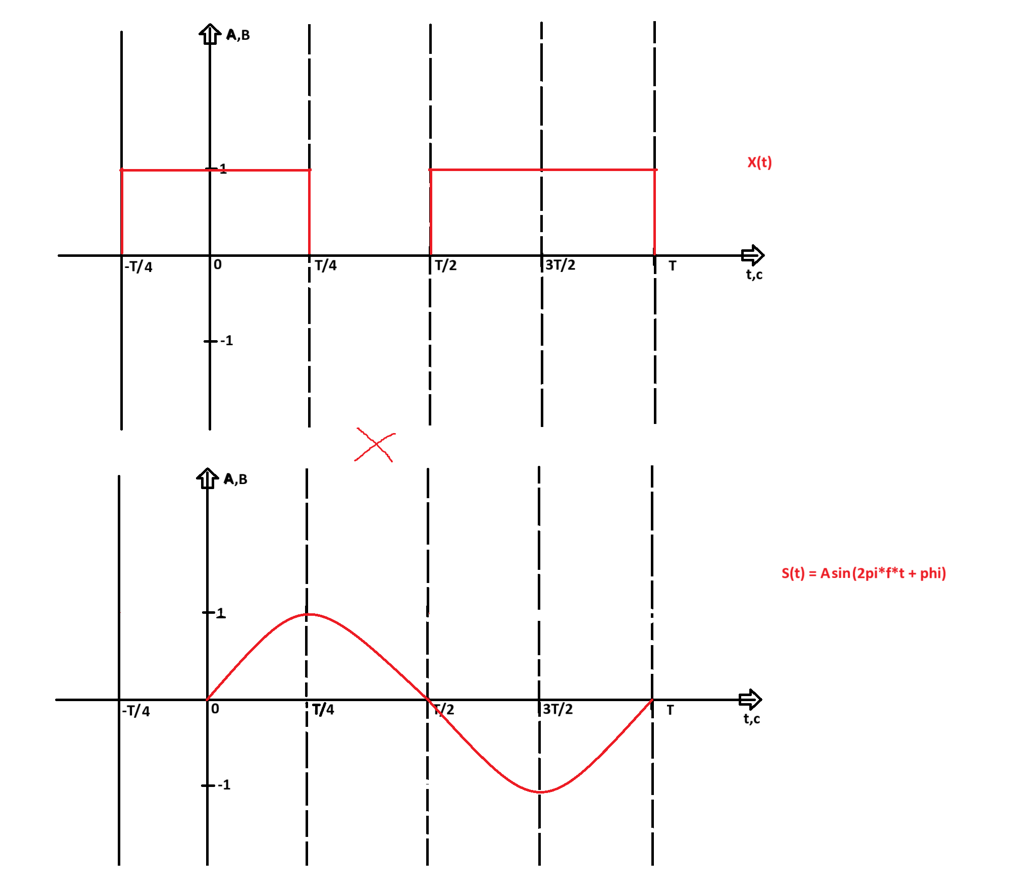
\includegraphics[width=1.0\textwidth]{b_comp_1.png}
    \caption{Геометрическая интерпретация вычисления $b_k$}
\end{figure}


\begin{figure}[H]
    \centering
    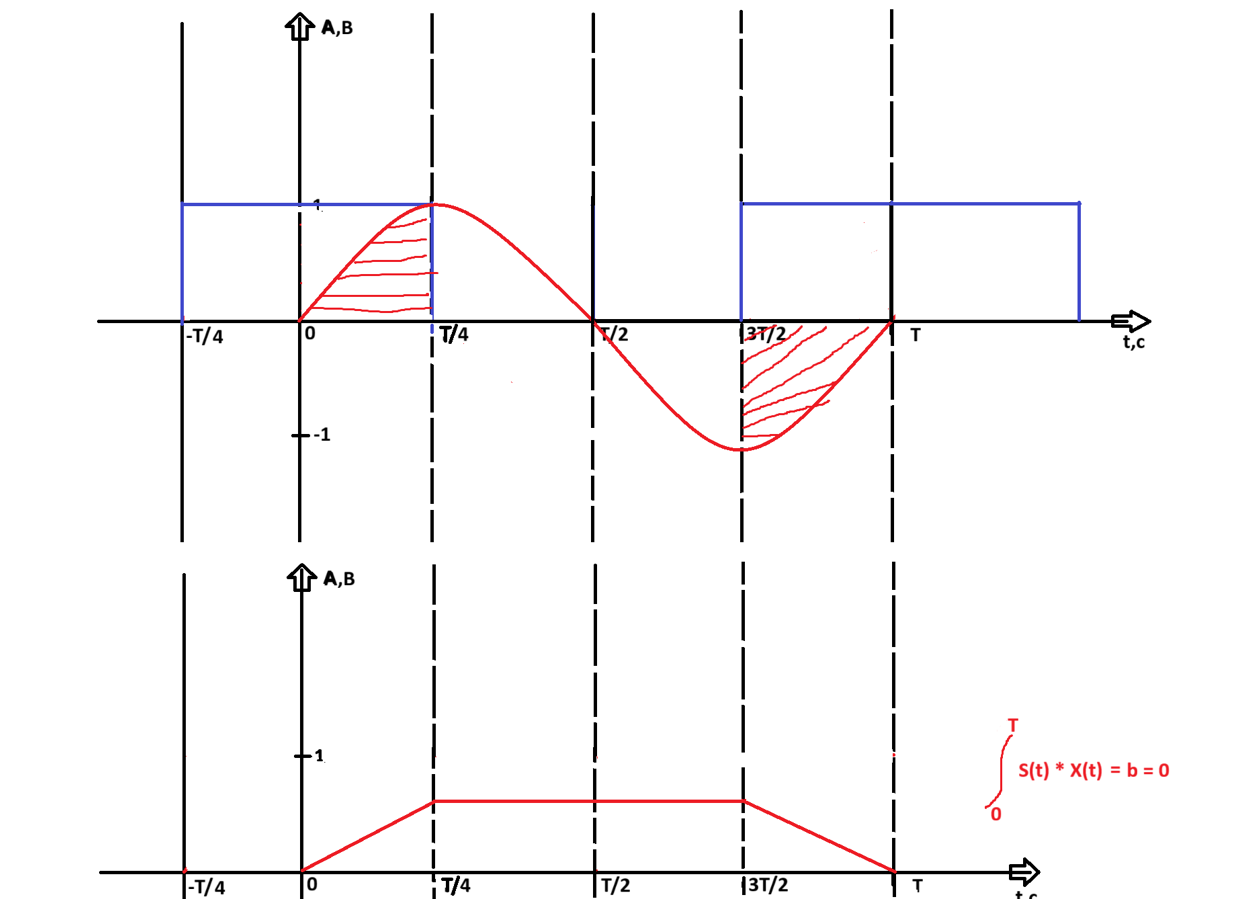
\includegraphics[width=1.0\textwidth]{b_comp_2.png}
    \caption{Геометрическая интерпретация вычисления $b_k$}
\end{figure}

Заметим, что исходный сигнал (прямоугольный) - четный, поэтому коэффциенты $b_k$ будут всегда равны нулю и в разложении
будет участвовать только cos($\omega_0t$)

\endinput